\section{Closeups and alerts}\label{closeups-and-alerts}

We describe here an approach which may provide a framework for relevant
and informative ICU alerts. ICU alerts are both not sufficiently
relevant (false alerts) and not sufficiently informative (trivial
alerts). ICU staff tends to ignore alerts because the alert often either
does not require an action, or the action will be taken anyway, with or
without the alert.

We introduce distinction between \emph{closeups} and \emph{alerts}. A
\emph{closeup} is a short timespan with observations which may require
attention. The computer finds closeups but does not force attention to
closeups per se. An \emph{alert} is the \emph{decision} that a closeup
does require human attention. Based on this decision, the computer may
light a bulb, play a sound, or draw attention in another way.

Many --- most --- closeups may be irrelevant. It is important though
that:

\begin{itemize}
\tightlist
\item
  Closeups are more often relevant than a random timespan.
\item
  It is easier to decide on a closeup's relevance than on a random
  timespan.
\item
  Closeups are hard to spot. One needs a tool to find and investigate
  them.
\end{itemize}

Most alerts, however, must be \emph{relevant}, \emph{actionable}, and
\emph{non-trivial}. * Relevant --- related to a change in condition
which requires attention. * Actionable --- the change in condition must
be easily deduced from the information supplied with the alert. *
Non-trivial --- the action following the alert would not be taken if the
alert were not issued.

\subsection{A model of early deterioration
signs}\label{a-model-of-early-deterioration-signs}

\begin{figure}[htbp]
\centering
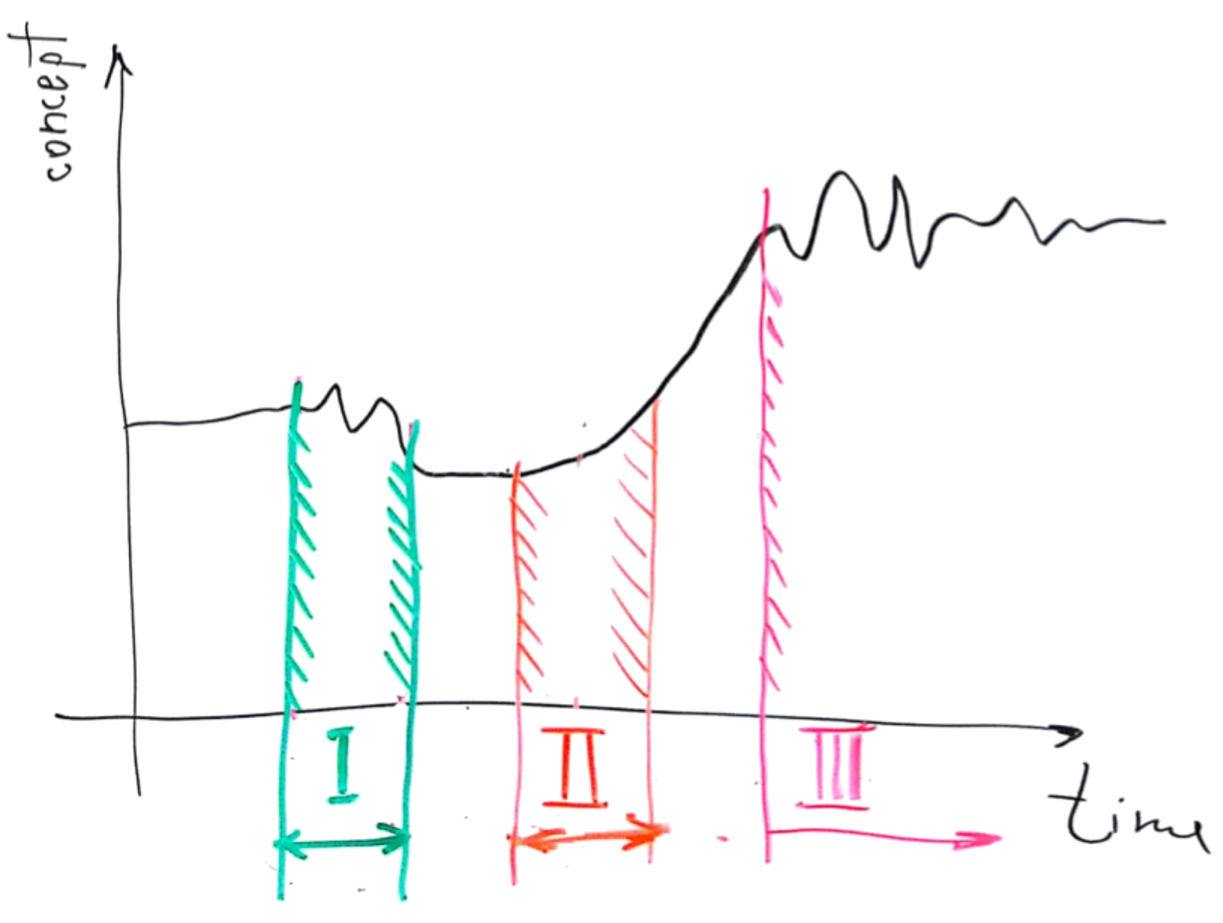
\includegraphics{deterioration-model.pdf}
\caption{Deterioration model}
\end{figure}

\subsection{Two-stage versus
end-to-end}\label{two-stage-versus-end-to-end}

\subsection{Locating closeups}\label{locating-closeups}

\subsection{Closeup features}\label{closeup-features}

\subsection{Deciding when a closeup is worth an
alert}\label{deciding-when-a-closeup-is-worth-an-alert}

\subsection{Early results}\label{early-results}
